\documentclass[10pt]{article}
\usepackage{fullpage,subfigure,fancyhdr}
\usepackage[pdftex]{color}
\usepackage{textcomp}
\usepackage{verbatim}
\usepackage{times}
\usepackage{amsfonts,amsmath,amssymb,amsthm}
\usepackage{textcomp}
\usepackage{url}
\usepackage{mdwlist}
\usepackage{wrapfig,caption,subfigure,sidecap}
\usepackage{xspace}
\usepackage{algorithm,algorithmic}
\usepackage[pdftex]{graphicx}
\usepackage[colorlinks=true,pagebackref,linkcolor=magenta]{hyperref}
\usepackage[sort&compress,comma,square,numbers]{natbib}
\usepackage{pict2e}
\usepackage[nottoc,numbib]{tocbibind}
\usepackage{paralist}
\usepackage{multicol}
\usepackage{lettrine}
\usepackage{helvet}
\usepackage{listings}
\usepackage[linecolor=dark_blue, linewidth=1.5pt, skipabove=4pt, nobreak=true]{mdframed}

% \usepackage{trackchanges}
% \usepackage{mcode}

\renewcommand{\familydefault}{\sfdefault}
\definecolor{MyGray}{rgb}{0.7,0.7,0.7}

% \numberwithin{figure}{section}
% \numberwithin{table}{section}
% \numberwithin{algorithm}{section}

\pagestyle{fancy}
% \oddsidemargin=-0.5in 
% \evensidemargin=-0.5in
\textwidth=6.5in 
\headwidth=6.5in
\textheight=9.0in 
\headheight=0.0pt
\topmargin=-0.5in
\headsep=0.2in
\renewcommand{\headrulewidth}{0pt}

\setlength{\parindent}{0em}
\setlength{\parskip}{0.5em}

%%%%% COLOR STUFF %%%%%%%%%%
\newcommand{\db}[1]{{\color{dark_blue}{#1}}}
\newcommand{\bb}[1]{{\textbf{\db{#1}}}}
\newcommand{\cb}[1]{\centering{{\textbf{\db{#1}}}}}

\definecolor{MyPlum}{rgb}{0.3,0,0.3}
\definecolor{MyOrange}{rgb}{1,0.5,0}
\definecolor{deep_blue}{rgb}{0,.2,.5}
\definecolor{dark_blue}{rgb}{0,.15,.5}

\newcommand{\marta}[1]{{\color{red}{\it marta: #1}}}
\newcommand{\youngser}[1]{{\color{green}{\it youngser: #1}}}
\newcommand{\brett}[1]{{\color{blue}{\it brett says: #1}}}
\newcommand{\jovo}[1]{{\color{magenta}{\it JoVo: #1}}}
\newcommand{\rb}[1]{{\color{red}{\it rb: #1}}}
\newcommand{\bro}[1]{{\color{blue}{\it youngser: #1}}}
\newcommand{\agastya}[1]{{\color{red}{\it agastya: #1}}}
\providecommand{\tg}[1]{\textcolor{green}{#1}}
\providecommand{\tb}[1]{\textcolor{blue}{#1}}
\providecommand{\tr}[1]{\textcolor{red}{#1}}
\providecommand{\tk}[1]{\textcolor{black}{#1}}
\providecommand{\twhite}[1]{\textcolor{white}{#1}}


%%%%%%%%% MATH OPERATORS %%%%%%%%%%%%
\providecommand{\ve}[1]{\boldsymbol{#1}}
\providecommand{\ma}[1]{\boldsymbol{#1}}
\providecommand{\norm}[1]{\left \lVert#1 \right  \rVert}
\providecommand{\deter}[1]{\lvert #1 \rvert}
\providecommand{\abs}[1]{\left \lvert #1 \right \rvert}
\providecommand{\mat}[1]{\left[ #1 \right]}
\newcommand{\trans}[1]{{#1}^{\ensuremath{\mathsf{T}}}}           % transpose
\newcommand{\transpose}[1]{{#1}^{\ensuremath{\mathsf{T}}}}           % transpose
\newcommand{\argmax}{\operatornamewithlimits{argmax}}
\newcommand{\argmin}{\operatornamewithlimits{argmin}}
\newcommand{\T}{^{\ensuremath{\mathsf{T}}}}           % transpose
\newcommand{\from}{{\ensuremath{\colon}}}           % :
\newcommand{\trace}[1]{{\ensuremath{\operatorname{tr}\!\left(#1\right)}}}           % :

\providecommand{\ms}[1]{\mathsf{#1}}
\providecommand{\mc}[1]{\mathcal{#1}}
\providecommand{\mt}[1]{\widetilde{#1}}
\providecommand{\mb}[1]{\boldsymbol{#1}}
\providecommand{\mbb}[1]{\mathbb{#1}}
\providecommand{\mv}[1]{\vec{#1}}
\providecommand{\mh}[1]{\hat{#1}}
\providecommand{\wh}[1]{\widehat{#1}}
\providecommand{\mhv}[1]{\mh{\mv{#1}}}
\providecommand{\mvh}[1]{\mv{\mh{#1}}}
\providecommand{\mhc}[1]{\hat{\mathcal{#1}}}
\providecommand{\mbc}[1]{\mb{\mathcal{#1}}}
\providecommand{\mvc}[1]{\mv{\mathcal{#1}}}
\providecommand{\mtc}[1]{\widetilde{\mathcal{#1}}}
\providecommand{\mth}[1]{\mt{\mh{#1}}}
\providecommand{\mht}[1]{\mh{\mt{#1}}}
\providecommand{\mhb}[1]{\hat{\boldsymbol{#1}}}
\providecommand{\whb}[1]{\widehat{\boldsymbol{#1}}}
\providecommand{\mvb}[1]{\vec{\boldsymbol{#1}}}
\providecommand{\mtb}[1]{\widetilde{\boldsymbol{#1}}}
\providecommand{\mbt}[1]{\widetilde{\boldsymbol{#1}}}
\providecommand{\mvc}[1]{\vec{\mathcal{#1}}}
% \newcommand{\D}[2]{\frac{\partial #1}{\partial #2}}
\newcommand{\dd}[2]{\frac{\partial ^2 #1}{\partial #2 ^2}}
\newcommand{\DDD}[3]{\frac{\partial ^2 #1}{\partial #2 \partial #3}}
\newcommand{\Di}[2]{\frac{\partial ^i #1}{\partial #2 ^i}}



%%%%%%%%%% ENVIRONMENTS %%%%%%%%%%%%%

\newtheorem{Rem}{Remark}%[section]
\newtheorem{Alg}{Algorithm}%[section]
\newtheorem{thm}{Theorem}
\newtheorem{Thm}{Theorem}[section]
\newtheorem{lem}{Lemma}
\newtheorem{Lem}{Lemma}%[section]
\newtheorem{defi}{Definition}
\newtheorem{Def}{Definition}[section]
\newtheorem{prop}{Proposition}
\newtheorem{coro}[thm]{Corollary}
\newtheorem{claim}{Claim}
\newtheorem{conj}{Conjecture}
\newtheorem{question}{Question}
\newtheorem{answer}{Answer}
\newtheorem{rem}{Remark}%[section]
\newtheorem{cor}[lem]{Corollary}
\newtheorem{model}{Model}
\newtheorem{remark}{Remark}

\newcommand{\bla}{\begin{block}}
\newcommand{\blb}{\end{block}}

\newcommand{\defa}{\begin{defi}}
\newcommand{\defb}{\end{defi}}
\newcommand{\theHalgorithm}{\arabic{algorithm}}

\newcommand{\thma}{\begin{thm}}
\newcommand{\thmb}{\end{thm}}

\newcommand{\mata}{\begin{bmatrix}}
\newcommand{\matb}{\end{bmatrix}}

\floatname{algorithm}{Procedure}
\renewcommand{\algorithmicrequire}{\textbf{Input:}}
\renewcommand{\algorithmicensure}{\textbf{Output:}}
\floatname{algorithm}{Pseudocode}



%%%%%%%%%% SECTIONS & STUFF %%%%%%%%%%%%%


\renewcommand{\thesection}{\Roman{section}}   % set the section counter to Alpha
\renewcommand{\thesubsection}{\Roman{section}.\Alph{subsection}}   % set the subsection counter to alpha
\renewcommand{\thesubsubsection}{\Roman{section}.\Alph{subsection}(\arabic{subsubsection})}   % set the subsection counter to alpha
% 
% 
\makeatletter
% \def\subsize{\@setsize\subsize{8pt}\xipt\@xipt}
 \def\section{\@startsection {section}{1}{\z@}{5pt}{9pt}{\Large\bf\db}}
 \def\subsection{\@startsection {subsection}{2}{\z@}{10pt}{4pt}{\large\bf\db}}
 \def\subsubsection{\@startsection {subsubsection}{2}{\z@}{10pt}{4pt}{\bf\db}}
% \def\subs{\@startsection {subsubsection}{2}{0pt}{5pt}{0pt}{ \subsize\bf\db}}
\def\paragraph{\@startsection {paragraph}{2}{\z@}{10pt}{4pt}{\bf\db}}
% \def\subparagraph{\@startsection 


\newcommand{\para}[1]{\vspace{3pt}\noindent{{\fontsize{10pt}{0pt}\bf\db{#1}}}}
\newcommand{\subpara}[1]{\vspace{3pt}\noindent{{\fontsize{10pt}{4pt} \bf \emph{#1}}}}
\newcommand{\subsubpara}[1]{\vspace{3pt}\noindent{{\fontsize{10pt}{4pt} \emph{#1}}}}

\setlength{\parindent}{0pt}



%%%%%% SHORT HAND %%%%%%%%%%
\renewcommand{\refname}{References and Notes}

\newcommand{\jv}{Joshua Vogelstein}
\newcommand{\jhu}{Johns Hopkins University}
\newcommand{\website}{http://jovo.me/}
\newcommand{\email}{jovo@jhu.edu}

\newcommand{\Vr}{V_{reset}}
\newcommand{\Vl}{V_{leat}}
\newcommand{\eqdef}{\overset{\triangle}{=}}
\newcommand{\grad}{\nabla}
\newcommand{\Hess}{\nabla\nabla}
\newcommand{\defn}{\overset{\triangle}{=}}

\newcommand{\iid}{\overset{iid}{\sim}}
\newcommand{\knn}{$k$NN}

\newcommand{\elegans}{\emph{C. elegans} }

\newcommand{\Lik}{\mathcal{L}}
\newcommand{\Cae}{[\widehat{\text{Ca}}^{2+}]}
\newcommand{\Cav}{\ve{C}}%[\ve{\text{Ca}}^{2+}]}
\newcommand{\sml}{\sqrt{\ma{\lambda}}}
\newcommand{\ml}{\ma{\lambda}}
\newcommand{\nw}{\widehat{n}}
\newcommand{\nv}{\vec{n}}
\newcommand{\Ae}{\widehat{A}}
\newcommand{\te}{\widehat{\tau}}
\newcommand{\maxn}{\max_{\ve{n}: n_t \geq 0}}
% \newcommand{\V}{\text{Var}}

\newcommand{\PmcP}{P \in \mc{P}}
\newcommand{\mP}{\mathbb{P}}

% \newcommand{\dvs}{\dot{\bs}_t}
% \newcommand{\dvw}{\dot{\bw}_t}
% \newcommand{\dvx}{\dot{\bx}_t}
% \newcommand{\dvy}{\dot{\by}_t}

\newcommand{\ft}{f_{\ve{\thet}}}
\newcommand{\gt}{g_{\ve{\thet}}}
\newcommand{\hht}{h_{\thetn}}

\newcommand{\Real}{\mathbb{R}}


\newcommand{\wconv}{\overset{i.p.}{\rightarrow}}
\newcommand{\sconv}{\overset{i.p.}{\rightarrow}}
\newcommand{\conv}{\rightarrow}
\newcommand{\pconv}{\overset{p}{\conv}}
\newcommand{\mcE}{\mathcal{E}}
\newcommand{\mcT}{\mathcal{T}}
\newcommand{\mcG}{\mathcal{G}}
\newcommand{\mcM}{\mathcal{M}}
\newcommand{\mcL}{\mathcal{L}}
\newcommand{\hatmcE}{\widehat{\mcE}}
\newcommand{\hatp}{\widehat{p}}
\newcommand{\hatP}{\widehat{P}}
\newcommand{\hatQ}{\widehat{Q}}
\newcommand{\hatL}{\widehat{L}}
\newcommand{\mhP}{\widehat{\PP}}
\newcommand{\tildeA}{\widetilde{A}}
\newcommand{\defeq}{\overset{\triangle}{=}}


\DeclareMathOperator{\Pmat}{\mathbf{P}}
\DeclareMathOperator{\veta}{\mathbf{\mb{v}}}
\DeclareMathOperator*{\minimize}{\mathrm{minimize}}
\DeclareMathOperator*{\maximize}{\mathrm{maximize}}
% \DeclareMathOperator*{\mb{v}mod}{\mathbf{\mb{v}}}


%%%%%%% LATIN LETTERS


\newcommand{\bA}{\mb{A}}
\newcommand{\bB}{\mb{B}}
\newcommand{\bD}{\mb{D}}
\newcommand{\bE}{\mb{E}}
\newcommand{\bI}{\mb{I}}
\newcommand{\bP}{\mb{P}}
\newcommand{\bS}{\mb{S}}
\newcommand{\bU}{\mb{U}}
\newcommand{\bV}{\mb{V}}
\newcommand{\bW}{\mb{W}}
\newcommand{\bX}{\mb{X}}
\newcommand{\bY}{\mb{Y}}
\newcommand{\bZ}{\mb{Z}}

\newcommand{\ba}{\mb{a}}
\renewcommand{\ba}{\mb{b}}
\newcommand{\bd}{\mb{d}}
\newcommand{\be}{\mb{e}}
\newcommand{\bp}{\mb{p}}
\newcommand{\bs}{\mb{s}}
\newcommand{\bu}{\mb{u}}
\newcommand{\bv}{\mb{v}}
\newcommand{\bw}{\mb{w}}
\newcommand{\bx}{\mb{x}}
\newcommand{\by}{\mb{y}}
\newcommand{\bz}{\mb{z}}


\newcommand{\Aa}{\mathbb{A}}
\newcommand{\BB}{\mathbb{B}}
\newcommand{\CC}{\mathbb{C}}         
\newcommand{\DD}{\mathbb{D}}         
\newcommand{\EE}{\mathbb{E}}           % expected value
\newcommand{\FF}{\mathbb{F}}         
\newcommand{\GG}{\mathbb{G}}
\newcommand{\HH}{\mathbb{H}}         
\newcommand{\II}{\mathbb{I}}           % indicator function
\newcommand{\LL}{\mathbb{L}}
\newcommand{\MM}{\mathbb{M}}
\newcommand{\NN}{\mathbb{N}}
\newcommand{\PP}{\mathbb{P}}         
\newcommand{\QQ}{\mathbb{Q}}           
\newcommand{\SSS}{\mathbb{S}}           
\newcommand{\VV}{\mathbb{V}}
\newcommand{\WW}{\mathbb{W}}         
\newcommand{\XX}{\mathbb{X}}         
\newcommand{\YY}{\mathbb{Y}}
\newcommand{\ZZ}{\mathbb{Z}}         




\newcommand{\Qs}{Q}
\newcommand{\mcS}{\mc{S}}
\newcommand{\mcU}{\mc{U}}

\newcommand{\mbd}{\mb{d}}
\newcommand{\mbD}{\mb{D}}
\newcommand{\mbx}{\mb{x}}
\newcommand{\mbX}{\mb{X}}
\newcommand{\mby}{\mb{y}}
\newcommand{\mbY}{\mb{Y}}

\newcommand{\mtbd}{\mtb{d}}
\newcommand{\mtbD}{\mtb{D}}
\newcommand{\mtbx}{\mtb{x}}
\newcommand{\mtbX}{\mtb{X}}
\newcommand{\mtby}{\mtb{y}}
\newcommand{\mtbY}{\mtb{Y}}



\DeclareMathOperator{\Ri}{\mathbf{\R}^{-1}}
\DeclareMathOperator{\A}{A}
\DeclareMathOperator{\W}{\mathbf{W}}
\DeclareMathOperator{\V}{\mathbf{V}}
\DeclareMathOperator{\U}{\mathbf{U}}
\DeclareMathOperator{\C}{\mathbf{C}}
\DeclareMathOperator{\uvec}{\mathbf{u}}
\DeclareMathOperator{\D}{\mathbf{D}}
\DeclareMathOperator{\Q}{\mathbf{Q}}
\DeclareMathOperator{\R}{R} %\mathbf{P}}
\DeclareMathOperator{\Y}{\mathbf{Y}}
\DeclareMathOperator{\B}{\mathbf{B}}
\DeclareMathOperator{\Hmat}{\mathbf{H}}
\DeclareMathOperator{\Gmat}{\mathbf{G}}
\DeclareMathOperator{\X}{\mathbf{X}}
\DeclareMathOperator{\Cmat}{C} %\mathbf{L}}\providecommand{\ms}[1]{\mathsf{#1}}

\DeclareMathOperator*{\Ymod}{\mathbf{\Y}}
\DeclareMathOperator*{\Bmod}{\mathbf{B}}
\DeclareMathOperator*{\Hmod}{\mathbf{H}}
\DeclareMathOperator*{\Lmod}{\mathbf{L}}
\DeclareMathOperator*{\Xmod}{\mathbf{\X}}


%%% THETA %%%%

\newcommand{\bth}{\ve{\theta}}
\newcommand{\hth}{\mh{\theta}}
\newcommand{\htth}{\mh{\theta}}
\newcommand{\bhth}{\mh{\ve{\theta}}}
\newcommand{\thetn}{\ve{\theta}}
\newcommand{\thet}{\thetn}
\newcommand{\theth}{\widehat{\ve{\theta}}}
\newcommand{\theto}{\ve{\theta}'}
\newcommand{\wht}{\widehat{\thet}}
\newcommand{\wtt}{\widetilde{\thet}}
\newcommand{\vth}{\ve{\thet}}
\newcommand{\vTh}{\ve{\Theta}}
\newcommand{\hvth}{\widehat{\ve{\thet}}}
\newcommand{\bTh}{\ve{\Theta}}
\newcommand{\hbth}{\widehat{\thet}}
\newcommand{\tbth}{\tilde{\bth}}



% \newcommand{\p}{P_{\bth}}
\newcommand{\pold}{P_{\bth'}}
\newcommand{\pk}{P_{\widehat{\ve{\theta}}^{(k)}}}
\newcommand{\pT}{P_{\thetn_{Tr}}} %\thetn_T
\newcommand{\pO}{P_{\thetn_o}} %\thetn_o
% \newcommand{\Q}{Q(\thetn,\theto)}
% \newcommand{\m}{m^{\ast}}
% \newcommand{\q}{q(\ve{H}_t)}
\newcommand{\Ca}{[\text{Ca}^{2+}]}


%%%%%% GREEK LETTERS

\newcommand{\del}{\delta}
\newcommand{\sig}{\sigma}
\newcommand{\lam}{\lambda}
\newcommand{\gam}{\gamma}
\newcommand{\eps}{\varepsilon}

\newcommand{\Del}{\Delta}
\newcommand{\Sig}{\Sigma}
\newcommand{\Lam}{\Lambda}
\newcommand{\Gam}{\Gamma}

\newcommand{\bSig}{\ve{\Sigma}}
\newcommand{\bOm}{\ve{\Omega}}
\newcommand{\bLam}{\ve{\Lambda}}
\newcommand{\bPhi}{\ve{\Phi}}
\newcommand{\bPsi}{\ve{\Psi}}

\newcommand{\bmu}{\ve{\mu}}
\newcommand{\bal}{\ve{\alpha}}
\newcommand{\bpi}{\ve{\pi}}
\newcommand{\bkap}{\ve{\kappa}}
\newcommand{\bdel}{\ve{\delta}}
\newcommand{\bphi}{\ve{\phi}}
\newcommand{\bpsi}{\ve{\psi}}



\DeclareMathOperator{\Delti}{\mathbf{\Delta}^{-1}}
\DeclareMathOperator{\Delt}{Q} %\mathbf{\Delta}}
% \DeclareMathOperator{\Gam}{\mathbf{\Gamma}}
\DeclareMathOperator{\Gami}{\mathbf{\Gamma}^{-1}}
\DeclareMathOperator{\Sigb}{\mathbf{\Sigma}}






%%%%%%%%%%% ALGORITHM NAMES %%%%%%%%%%%%%


\providecommand{\sct}[1]{{\sc \texttt{#1}}}

\newcommand{\Idt}{\sct{Idt}}
\newcommand{\Svd}{\sct{Svd}}
\newcommand{\Svm}{\sct{Svm}}
\newcommand{\Pca}{\sct{Pca}}
\newcommand{\Fld}{\sct{Fld}}
\newcommand{\Lda}{\sct{Lda}}
\newcommand{\eig}{\sct{eig}}
\newcommand{\Lol}{\sct{Lol}}
\newcommand{\Lal}{\sct{Lal}}
\newcommand{\Qoq}{\sct{Qoq}}
\newcommand{\Lrl}{\sct{Lrl}}
\newcommand{\Lfl}{\sct{Lfl}}
\newcommand{\Faq}{\sct{Faq}}
\newcommand{\qr}{\sct{qr}}
\newcommand{\FoP}{\Fld$\circ$\Pca}
\newcommand{\PoF}{\Fld$\circ$\Pca}
\newcommand{\Road}{\sct{Road}}
\newcommand{\Mgc}{\sct{Mgc}}






\usepackage{caption}
\usepackage{wrapfig}

\pagestyle{fancy}
% \oddsidemargin=-0.5in 
% \evensidemargin=-0.5in
\textwidth=6.5in 
\headwidth=6.5in
\textheight=9.0in 
\headheight=0.5pt
\topmargin=-0.5in
\headsep=0.5in
% \rhead{\textsf{\color{MyGray}{RESEARCH ARTICLES}}}
% 

% \usepackage[landscape,margin=1in]{geometry}% http://ctan.org/pkg/geometry
% \usepackage{flowfram}% http://ctan.org/pkg/flowfram
\usepackage{helvet}
\renewcommand{\familydefault}{\sfdefault}

% First page setup    
% \newstaticframe[1]{0.63\textwidth}{0.35\textheight}{0.02\textwidth}{0.65\textheight}[titleabstract]
% \newflowframe[1]{0.30\textwidth}{0.65\textheight}{0.02\textwidth}{0pt}[shortleftcolumn]
% \newflowframe[1]{0.30\textwidth}{0.65\textheight}{0.35\textwidth}{0pt}[shortcentercolumn]

% % Subsequent pages setup    
% \newflowframe[>1]{0.3\textwidth}{\textheight}{0.00\textwidth}{0pt}[leftcolumn]
% \newflowframe[>1]{0.3\textwidth}{\textheight}{0.32\textwidth}{0pt}[centercolum]
% \newflowframe[all]{0.3\textwidth}{\textheight}{0.67\textwidth}{0pt}[rightcolumn]
% \newstaticframe[2]{0.63\textwidth}{0.5\textheight}{0\textwidth}{0.3\textheight}[lefttwo]


% \Ncolumntop[2]{flow}{2}{4in}

\title{\vspace{-50pt}LOL Extra}
\author{Joshua T.~Vogelstein, Mauro Maggioni}
\date{}

\begin{document}
\maketitle

% \section{Introduction}

% Opening:
As scientific measurements become increasing easy and inexpensive to obtain, the dimensionality of scientific data is exploding.  Common examples include genomics, wherein an individual is encoded by a 6 billion dimensional sequence, and connectomics, wherein an individual is encoded by up to 1 million nodes, and therefore up to $10^{12}$ potential interaction terms.  Such rich representations provide hope for mining these data to find, for example, prognostic biomarkers or personalized therapies.  That said, utilizing these data at their native resolution and dimensionality has been hindered thus far.

% Challenge
The most pernicious impediment is perhaps the low sample size relative to the number of observed dimensions:  while the observed dimensionality has ballooned, the sample sizes have \emph{not} witnessed a concomitant increase.  It is common for sample sizes to be in the tens; hundreds is considered a very large experiment, and thousands is all but unheard of (see, for example, Table 2 of \cite{DiMartino2014} in connectomics, and XXX in genomics).   This means that we often do not have a large enough sample size to obtain high power (or accuracy) without assuming some additional structure in the data. 
In other words, even though the information is likely present in the high dimensional data, our ability to discover it is impeded. 
To combat this problem, we can assume some structure, and then use that assumption to significantly reduce the number of parameters to estimate.  
Although the set of such possible assumptions is vast, we characterize all such options into one of three philosophical methodologies.


One recently very popular approach is to assume sparsity, that is, that a small subset of the observed dimensions contain sufficient information to make quality predictions \cite{Olshausen97a, Buhlmann2014}.  Sparse methods include screening methods such as higher criticism screening \cite{Donoho08a}, L1 penalized methods such as LASSO \cite{Tibs96}, and more recent sparse discriminant analysis methods \cite{Clemmensen2011,Mai12a,Fan2012}. While very useful because they admit readily interpretable results, they are guaranteed to work only in very restricted situations \cite{Buhlmann2014}.  Specifically, they require certain orthogonality conditions on the individual dimensions (or features), and require that a small number of those features have large predictive accuracy.  


Another alternative is to ``pre-process'' the data via applying some unsupervised manifold learning technique, which search for a low dimensional representation.  The most well-known such example of such a methodology is principle components analysis (PCA) \cite{Pearson1901,Hotelling1933}.  In the $>$110 years since its original development, many extensions and generalizations of PCA have been proposed, including random projections \cite{Candes06a}, NMF \cite{Paatero94a, LeeSeung99}, and kernel variants of PCA such as isomap \cite{Tenenbaum2000}, LLE \cite{Roweis2000}, and Laplacian Eigenmaps \cite{Belkin2003}. These methods can find more general representations than their sparse counterparts by discovering linear or nonlinear combinations of the observed dimensions to represent the data.  However, these approaches do not utilized the supervised information to discover the best representation for accurate predictions or tests.  Thus, even though they sometimes provide strong theoretical support for discovering the true underlying manifold under rather general settings \cite{deSilva2003,Allard12a}, the goal in this work is \emph{not} to find the \emph{true} manifold of the data, but rather, to find the manifold that maximizes accuracy.


We therefore consider a third philosophy, which we call supervised manifold learning.  This approach takes the best of both worlds from the previously mentioned approaches: it can in theory find very complex linear or nonlinear combinations of the original observed dimensions, and it does so in a fully supervised manner.  In fact, the two previous approaches can accurately be thought of as special cases of this more general approach (see Appendix for rigorous definitions).  A number of investigators have previously developed supervised manifold learning methods.  A set of methods from the statistics community is collectively referred to as   ``sufficient dimensionality reduction'' methods  \cite{Li1991, Cook91a, Globerson2003, Bouveyron07a, Cook08a}.  These methods are theoretically elegant, but typically require the sample size to be larger than the number of observed dimensions (although see \cite{Cook13a} for some promising work).  Other approaches formulate an optimization problem, such as projection pursuit \cite{Huber1985} or supervised dictionary learning \cite{Mairal2008}.  These methods are limited because they are prone to fall into local minima, they require costly iterative algorithms, and lack any theoretical guarantees \cite{Belkin2006}.  Thus, their remains a gap in the literature: a supervised learning method with theoretical guarantees under general conditions with an efficient algorithm.

% Action:
In this work, we present such a method, which we term LOL, for Low-rank Optimal Linear projection.  The key idea emerges from considering perhaps the simplest supervised learning task: a two-class classification problem.  It is immediate that even for multivariate Gaussian data, the discriminant boundary (that is, the boundary that discriminates between the two classes) is a function of both: (i) the difference of the means, and (ii) the covariance of the two classes.  Therefore, we find a low dimensional representation of the data utilizing both of these objects. 


% Resolution:
The simplicity of this idea translates into a methodology that readily admits theoretical investigation, efficient implementations, and generalizations.  We provide all of them in this work.  Moreover, we demonstrate improved performance over competing ideas in terms of both accuracy and speed, for a number of simulated and real data examples.  Moreover, straightforward extensions of this idea lead to similarly simple and useful other tasks, such as multi-class classification, regression and testing.  We provide open source MATLAB and R code to enable further extensions and applications.






\section*{Results}



\subsection*{The Generality of LOL}

To understand the generality of applicability of LOL, we consider possibly the simplest supervised manifold learning setting.  Specifically, we consider a two-class classification problem, where both class have multivariate Gaussian distributions.  To further simplify, we assume that the two classes have the same covariance, so that the only difference between the two classes are the means. 
Formally, we write $\mb{X} | Y=y \iid \mc{N}_D(\bmu_y, \bSig)$, where $\mb{X}$ is a $D$-dimensional vector of observed features, $y$ is a binary class label, $\iid$ indicates that each $\mb{X}$ is sampled identically and independently according to some distribution, and $\mc{N}_D(\bmu_y,\bSig)$ indicates a $D$-dimensional Gaussian distribution with mean $\bmu_y$ (different for the two classes) and covariance $\bSig$ (the same for the two classes).
In such a scenario,  the Bayes optimal classifier is Fisher's Linear Discriminant Analysis (LDA).  Specifically, the Bayes classifier projects a new sample, $\bx$, onto the subspace spanned by the dot product of the inverse covariance matrix with the difference of the mean vector:
\begin{align}
g_*(\bx) = 
\begin{cases}
      1 & \text{if}\ \bx\T \bSig^{-1} \mb{\delta} > t, \\
      0 & \text{otherwise},
    \end{cases} \label{eq:LDA}
\end{align}
\noindent where $\mb{\delta}=\bmu_0-\bmu_1$, and $t$ is a simple linear function of the class priors and the mean of the class means.  
Eq. \eqref{eq:LDA} shows that the optimal manifold for discriminating between two multivariate Gaussian distributions with the same covariance is a linear manifold spanned by $\bSig^{-1} \mb{\delta}$.  
From this, it would seem that any manifold learning methodology that we employ would benefit from including both an estimate of the mean difference, $\mhb{\delta}$, as well as the pooled covarianced, $\mhb{\Sigma}$.  Unsupervised manifold learning techniques ignore $\mhb{\delta}$, only utilizing $\mhb{\Sigma}$.  Sparse methods struggle with correlated data, that is, data for which the covariance matrix is dense in the off-diagonal elements.  This motivates the use of supervised manifold learning techniques that overcome these two problems.  

To illustrate the differences between these three methods, we consider three different parameter settings for the above specified model.  In each, we let $D$, the number of observed dimensions, be 1000, whereas we only sampled $n=100$ points total, so that $D \gg n$.  
Fisher's Linear Discriminant Analysis (LDA) would be optimal in these settings if the parameters were known or easily estimable, but because sample size equals the ambient dimension, the estimated covariance matrix is singular, and so LDA does not even run. Instead, therefore, we consider an example of three different methodological principles. 
For each method, we embed the data into five dimensions.  


First, we consider the simplest parameter setting: a single observation dimension contains nearly all the discriminant signal, and that dimension is the dimension of maximal variance (see Figure \ref{fig:cigars}(A)).  This situation is ideal for using PCA to pre-process the data, as PCA finds the directions of maximal variance.  However, PCA in high-dimensions is inconsistent, and has relatively high variance \cite{Cai2012,Fishkind2013a}.  Therefore, even in this idealized scenario, running LDA on the data projected onto the first 5 principal components yields subpar performance (second row of (A)).  On the other hand, because the signal is so sparse, a method designed specifically for sparse multivariate Gaussian classification (Regularized Optimal Affine Discriminant; ROAD \cite{Fan2012}), performs very well (third row of (A)).  Similarly, because LOL uses both the discriminant dimension and the principle components, LOL also does essentially optimally (fourth row of (A)).  Finally, we also show the Bayes optimal performance (bottom row of (A)) for comparison purposes.


Second, we consider a related parameter setting, but now, the dimension with most of the discrimination information is aligned with the dimension of maximal variance.  This is the worse possible scenario for using PCA to pre-process the data.  Unfortuantely for PCA, we can readily prove that this scenario is much more common than the prior scenario, under relatively general settings (see Appendix).




%  The first principle is unsupervised manifold learning, the most popular variant thereof being Principle Component Analysis (PCA).  The classifier we employ therefore first uses PCA to find an unsupervised low dimensional representation of the data, and the applied LDA in the projected space.  



% The second through fifth rows of this figure depict the estimated predictions of four different classifiers: (i) linear discriminant analysis (LDA) applied to the data projected into a low dimensional space via PCA; (ii) Regularized Optimal Affine Discriminant (ROAD) \cite{ROAD}, a recently described sparse method derived specifically for this kind of setting; (iii) LDA applied to the data after projecting into a lower dimensional space via Linear Optimal Low-rank (LOL), which is our newly developed supervised manifold learning method; and (iv) the Bayes classifier, which performs optimally.  

% In each of these four rows, the solid (dashed) line depicts the empirical distribution of predictions from class 0 (class 1),  thus, smaller filled area is better performance.


Column (A) depicts the simplest setting: the optimal one-dimensional discriminant boundary is aligned with the direction of maximal variance.  Thus, PCA finds this discriminant boundary,  sparse methods do as well, as does LOL. Column (B) depicts a slightly more difficult setting, the optimal one-dimensional discriminant boundary is aligned with the direction of minimal variance.   This is the most difficult setting for PCA, because PCA finds the directions of maximal variance, and thus discards directions of minimal variance (which, in this case, includes the optimal discriminant direction).  Sparse methods could recover the optimal discriminant direction, but typically fail to find it.  Rather, they find a random collection of other dimensions, each of which is equally and minimally informative.  LOL performs significantly better, as it is able to fuse information across multiple dimensions.  Finally, column (C) depicts the same setting as column (B), but all data have been randomly rotated.  Both LDA $\circ$ PCA and LOL are invariant to such rotations, so there expected performance does not change.  Sparse methods now randomly select a few dimensions, as each ambient dimension is now equally informative.  


\subsection*{Finding the Best (not the True) Manifold}


\subsection*{LOL for Wide Regression and Testing}


\section*{Discussion}



% \end{staticcontents*}

% \renewcommand{\familydefault}{\rmdefault}
% \tableofcontents
% \clearpage
% \section{Introduction}

% \begin{minipage}{2\linewidth}
% \begin{multicols}{2}
% {\noindent \Huge Supervised Manifold Learning for Big Scientific Data}
%  	
% \noindent \textbf{Joshua T.~Vogelstein$^{1,2}$, Mauro Maggioni$^1$}
%  
% \noindent To perform statistical inference on high-dimensional data, one can often improve finite sample performance on particular exploitation tasks via embedding the data into a lower-dimensional space.  Rather than first choosing a manifold learning algorithm and then composing it with a classification algorithm, we derive the form of the optimal affine subspace projection for the simplest case of interest: a  two-class classification problem in which both classes are sampled from multivariate Gaussian distributions.  Simulations demonstrate improvements over the previous state-of-the-art in performance in a variety of settings, at trivial additional cost.  The same intuition leads to a novel two-sample test in high-dimensions with higher power than the previous state-of-the-art.  Extensions to multiple classes and non-parametric extensions are straightforward.
% \end{multicols}
% \end{minipage}




% \begin{multicols}{3}


% \paragraph{Opening} 
\lettrine[lines=3]{B}{}ig data are abundant.  The applications of big data range from government, to industry, to science, with serious potential societal implications. Most big data analytics thus far, however, deal with huge sample size (e.g., $n=10^7$) and large  dimensionality (e.g., $p=10^4$).  Big scientific data, however, has the opposite characteristic: the dimensionality is huge (e.g., number of base pairs in a genome, or potential edges in a connectome), and the sample size is relatively small (e.g., hundreds typically). Optimally extracting information from such big scientific data therefore requires radically different approaches than typical industry or government big data problems.  We are particularly interested in ``supervised'' learning problems here, such as building a classifier that operates on a whole genome or connectome, to make a diagnosis. In such cases, the genome or connectome comprise the \emph{predictor} variables and the diagnosis represents the \emph{target} variable.


To gain insight into the challenges associated with big scientific data,  consider the MNIST dataset, consisting of images of the digits, 0-9 \cite{mnist}.  The top row of Figure \ref{fig:mnist} depicts four random samples of digits 3, 7, and 8 each. Our task is to learn a classifier $\hat{g}_n(\cdot)$ from a set of $n$ such samples, such that given a new image, $\hat{g}_n(\cdot)$ would accurately determine the true class of the image.  Each of these images is $28 \times 28$ pixels, meaning it has dimensionality $p=784$.  To make this scenario similar to the big scientific data scenario of interest, we have limited the number of training samples to $n=100$, so that $n \ll p$.  In such scenarios, it is well known that classic tools, such as linear discriminant analysis fail \cite{Bickel04a}, because we lack sufficient information to obtain reliable estimates of the parameters.  The statistics and machine learning communities have developed a number of mitigating strategies for such problems.  





One recently very popular approach is to assume sparsity, that is, that a small subset of the given dimensions contain sufficient information to make quality predictions \cite{Olshausen97a, Buhlmann14a}.  Sparse methods include screening methods such as higher criticism screening \cite{Donoho08a}, L1 penalized methods such as LASSO \cite{Tibs96}, and more recent sparse discriminant analysis methods \cite{Clemmensen2011,Mai12a,Fan2012}. These methods are inappropriate and inadequate for such applications, because there does not exist a small number of ambient dimensions that adequately capture the discriminant information.  This is evidenced by panel (D), which shows the most discriminating pixels, and panel (G) which shows 100 test images embedded into the top three dimensions discovered by a sparse approach. The three different classes are clearly not well distinguished, as quantified by the cyan line in panel (J), which shows the error rate (1-accuracy) for a variety of methods as a function of the number of embedded dimensions to keep.


Another alternative is to ``pre-process'' the data via applying some unsupervised manifold learning technique, which search for a low dimensional representation (potentially a manifold or collection thereof) of the predictor variables.  Examples of such approaches includes PCA \cite{Jolliffe2002}, random projections \cite{Candes06a}, NMF \cite{Paatero94a, LeeSeung99}, and LLE \cite{Roweis2000}.  Panel (E) shows the top four eigenimages of these data, that is, the four images that collectively capture the most variance of all possible four images.  Clearly, each image has aspects of 3, 7, and 8 in it, which is intuitively pleasing.  However, panel (H) shows 100 test images embedded into the top three such dimensions. Clearly, these data are again not very well separated, although much better separated than the sparse methods, as evidenced by the magenta line in panel (J).  




Finally, the philosophy that we adopt in our work can be characterized as a supervised manifold learning technique. Such techniques seek to utilize both the predictor dimensions as well as the target variables to discover a low dimensional representation of the discriminant boundary.  Sparse methods, are in fact, a special case of this approach, in which the discriminant boundary is assumed to lie along  a subset of the predictor variables.  More general supervised manifold learning techniques allow the low dimensional representation to be a (potentially nonlinear) combination of predictor variables.  ``Sufficient dimensionality reduction'' methods  \cite{Li1991, Cook91a, Globerson2003, Bouveyron07a, Cook08a}, while theoretically appealing, require the sample size to be larger than the ambient dimensionality  (although see \cite{Cook13a} for some promising work).  Other methods formulate an optimization problem, such as projection pursuit \cite{Huber1985} or supervised dictionary learning \cite{Mairal2008}.  These methods are limited because they are prone to fall into local minima, they require costly iterative algorithms, and lack any theoretical guarantees.  

Our approach is termed LOL, for Low-rank Optimal Linear projection.  On the MNIST dataset, the first few projection vectors that it learns look much like the unsupervised ones (see panel (F)); indeed, they are also linear combinations of the training samples. However, LOL results in embeddings that clearly separate the three classes (panel (I)).  The improvement in classification performance over the other methods is dramatic, as quantified by the green line in panel (J).  Moreover, computational time is just slightly longer than the unsupervised approach (panel (K)), and faster than the sparse method.

Our construction follows from a simple geometric argument given perhaps the simplest big scientific data supervised learning problem.  This intuition leads to a formulation that admits an approach that improves over the current state of the art along many factors, including clarity, ease of implementation, computational efficiency, scalability, and theoretical justification.  Moreover, its simplicity immediately leads to a number of extensions and generalizations.  We demonstrate its properties on a range of simulations and real data experiments.  Moreover, we provide open source MATLAB and R code to enable further extensions and applications.





\section*{Motivating Intuition}

To gain insight into the challenges associated with big scientific data,  we considered the simplest such problem we could think of: a two-class classification problem, where each class conditional distribution is a multivariate gaussian, and the classes have a shared covariance (see Figure \ref{fig:cigars}, top left panel).  


Figure \ref{fig:cigars} shows a couple examples with diagonal covariance matrices. Because the sample size ($n=50$) is significantly smaller than the ambient dimension ($p=100$), classical methods will fail.  Thus, a technique, such as the above, could potentially alleviate the issue.  However, this problem is difficult because  the principle direction of variance is \emph{orthogonal} to the principle discriminant direction.  Thus, unsupervised methods will discard the discriminant signal in favor of the variance dimensions.  Moreover, because the discriminant dimension is not a canonical dimension, but rather a linear combination thereof, sparse methods will also fail.  We therefore are left with supervised dictionary learning techniques.  When the dimensionality is large, F2M methods will fail, and iterative optimization methods will be too computationally burdensome.  


In such a scenario, a simple linear algebraic calculation reveals that the optimal projection matrix is the dot product of the difference between the means with the shared inverse covariance matrix, $\mb{\delta}\T \bSig^{-1}$.  However, when the number of dimensions $p$ is much greater than the number of samples $n$, we obtain estimates of $\bSig$ that are badly scaled, such that inverting the matrix is numerically unstable.  





% \begin{figure*}[htbp]
% 	\centering
% 		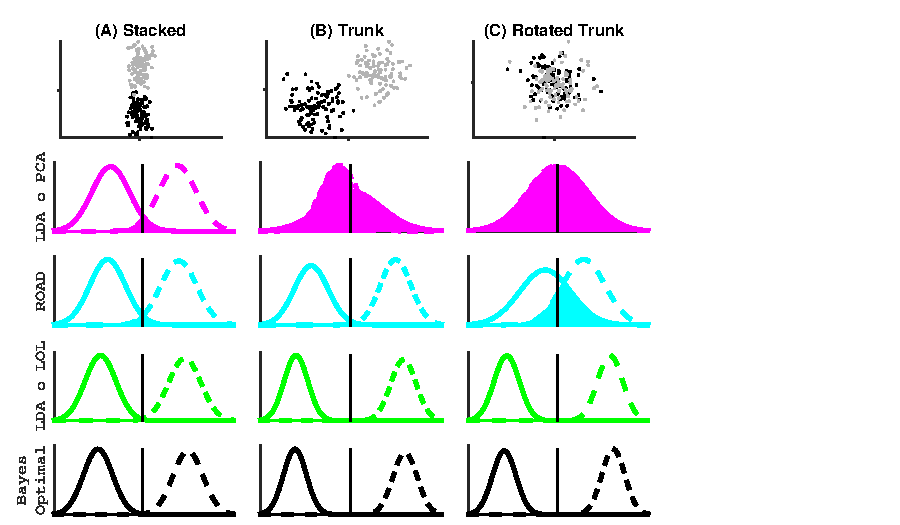
\includegraphics[width=1.0\linewidth, trim=0.8in 0in 0.4in 0in, clip]{../Figs/cigars.pdf}
% 	\caption{In certain situations, the top principal components can be orthogonal to the discriminant manifold (left column).  In such situations, dimension reduction via PCA will discard all of the signal, because PCA is a fully unsupervised dimension reduction technique (2nd column from left).  On the other hand, LOL estimates the discriminant manifold, which maintains most of the the signal (3rd column from left).  The Bayes classifier, of course, keeps all of the signal (4th column from left).  Key simulation parameters: $\#$ training samples: 50; ambient dimension: 100; intrinsic dimension: 1; $\#$ dimensions projected onto: 5.  Top: covariance matrix is the identity; Bottom: first dimension is rotated by 90$^\circ$. See Methods for more details.}
% 	\label{fig:cigars}
% \end{figure*}




\section{Results}

\subsection{Main Approach}

\subsection{Numerical Results}

% \clearpage
\paragraph{Illustrative example on real data}



% \clearpage
\paragraph{Generalizations}


% \begin{figure*}[htbp]
% 	\centering
% 		\includegraphics[width=1.0\linewidth]{../Figs/generalizations.pdf}
% 	\caption{Each panel shows misclassification (error) rate as a function of the number of embedded dimensions, with LOL (in green), as compared to other approaches. 
% 	% 
% 	% 
% % 	
% 	(A) low-d toeplitz: LOL vs. PCA, 
% 	(B) large-d toeplitz: LOL vs PCA
% 	(C) rotational invariance: LOL vs PCA
% 	(D) semisupervised: ssLOL, ssPCA
% % 
% 	(E) multiple subspaces: LOL vs QOL, LOQ, QOQ, 
% 	(F) robust: LOL vs. RoLOL
% 	(G) fast: LOL vs. FLOL vs RaLOL vs DRP	
% 	}
% 	\label{fig:generalizations}
% \end{figure*}

The simplicity of LOL enables a wide range of applications and extensions (Figure \ref{fig:generalizations}).  
\begin{enumerate}
	\item In the ``Trunk'' example, each of the 500 ambient dimensions contains signal, although the amount of signal is decreasing geometrically, while the variance is increasing geometrically.  With only 50 training samples, LDA$\circ$PCA never performs as well as LOL with only a single dimension. This example was originally proposed to demonstrate that the optimal number of dimensions to keep when estimating a classifier is a function of the sample size.  
	\item It is increasingly common to assume sparsity in the data.  Recent advances is sparse linear discriminant analysis demonstrate impressive theoretical and empirical results.  Four recently proposed methods include the $\ell_1$-Fisher's discriminant analysis (FSDA) \cite{Wu2008}, sparse optimal scoring  (SOS) \cite{Clemmensen2011}, direct sparse discriminant analysis (DSDA) \cite{Mai2012}, and regularized optimal affine discriminant (ROAD) \cite{Fan2012}.  \cite{MaiZou2013} proved that the first three are equivalent, and \cite{Mai2013} numerically compares them with ROAD, as well as nearest shrunken centroids (PAM) \cite{Tibshirani2002} and features annealed independence rules (FAIR) \cite{FanFan2008}.   While the first four use the correlation structure, the last two discard it, much like the na\"ive Bayes classifier as discussed in \cite{BickelLevina2004}.  \cite{Mai2013} showed that including covariance is useful.  All of these approaches, however, are rotationally sensitive.  That is, they all benefit from the data living in a sparse subset of the ambient bases, rather than a learned dictionary in that subspace.  In other words, all these methods suffer if the data are arbitrarily rotated.  To demonstrate this, we chose a simulation setting provided by \cite{Fan2012}, with $D=1000$ but $n=300$, and $s=10$ (number of signal dimensions) in which ROAD performs nearly optimally, and rotated the data by a random rotation matrix.  The performance of ROAD, as well as all the other algorithms, significantly deteriorates in this context.  On the other hand LOL is rotation invariant, and moreover, significantly faster than these other covariance dependent algorithms, as LOL utilizes extremely optimized numerical linear algebra routines such as \texttt{svd} and \texttt{qr}, whereas the other methods require relatively computationally intensive iterative optimization algorithms.  Because of this, LOL also scales up to millions or billions of dimensions, whereas none of the other methods have this level of scalability. 
	\item The third example we constructed to exhibit slower spectral decay than the previous ones, to reflect real data scenarios.  More specifically, the covariance matrix is Toeplitz, and the difference between the means is a square wave, which lives in the subspace spanned by the eigenvectors corresponding to the lowest eigenvalues.  Thus, this example corresponds to a difficult, but realistic, scenario.  For simplicity, we let $D=n=50$ in this example, although we can easily tune the parameters to yield identical performance for $D$ and $n$ of any size. 	 As (C) shows, LOL again significantly outperforms LDA$\circ$PCA in terms of misclassification rate for almost all embedding dimensions.  Moreover, both algorithms exhibit a noticeable unimodal shape, with misclassification rate improving as it keeps including more informative dimensions, and then begins to degrade as subsequent dimensions are more noise than signal.  
	\item The flexibility of LOL enables us to consider a wide range of extensions. Fast via randomized svd, or random projections
	
	\item Multiple subspaces
	
	\item Robust
	
	\item  In semi-supervised settings, many training samples may lack labels.  In such a scenario, we can still leverage the unlabeled samples to contribute to the pooled covariance estimate. Thus, under certain settings \cite{Yang2011a} we can improve performance via utilizing those additional data.  Panel (D) is the same setting as panel (C), but now we have 50 labeled samples, and an additional 450 unlabeled samples, thus only 10\% of the samples are labeled.  
\end{enumerate}


% \clearpage
\paragraph{Scalability}


% \clearpage
\paragraph{Novel Applications}


% \begin{figure}
% \centering
% 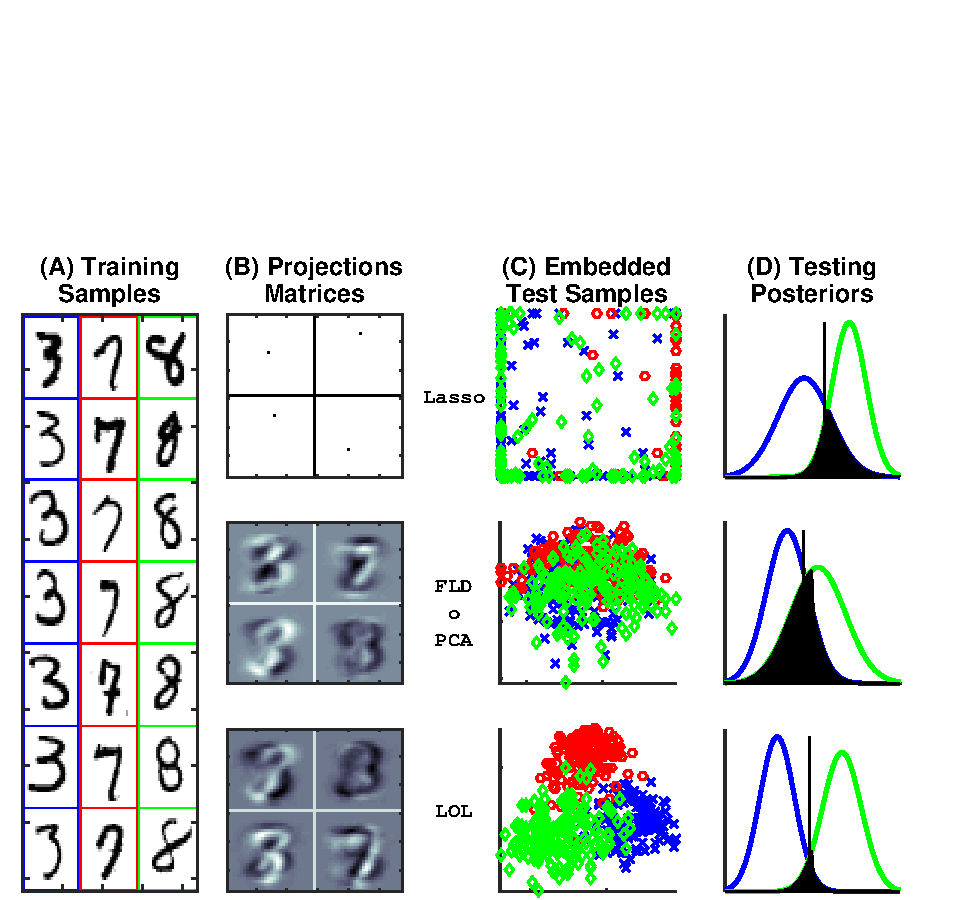
\includegraphics[width=1\linewidth, trim=0in 2in 0.5in 0, clip]{../Figs/mnist.pdf}
% \caption{In many real data applications, the difference of the means contains much of the discriminant manifold.  We subsampled 100 points from the MNIST dataset, consisting of the numbers 3, 7, and 8, and applied both LOL and PCA to embed the data into a small dimension.  Clearly, the first two dimensions of LOL (left panel) separate these data far better than the first few dimensions of PCA (middle panel).  This translates into vastly superior performance in subsequent classification (right panel).}
% \label{fig:mnist}
% \end{figure}


% \begin{figure*}[h!]
% 	\centering
% 		% \includegraphics[height=3in]{../../Figs/performance_toeplitzs.pdf}
% 	\caption{performance on new datasets, eg, ABIDE, Amen, cancer?}
% 	\label{fig:applications}
% \end{figure*}



% \clearpage
\subsection{Theoretical Results}




In particular, let $\rho$ denote the correlation between the mean difference vector and the diagonal of the diagonal covariance matrix.
Let $\rho_{PCA}(i)$ be the correlation between the Bayes optimal projection $\mb{A}_*$ and the i$^{th}$ eigenvector, and let $\rho_{LOL}(i)$ be defined similarly, for the $i^{th}$ projection vector of LOL.  Similarly, 
let $\theta_i$ be the correlation between the mean difference vector $\delta$ and the $i^{th}$ eigenvector.
Let the unsubscripted version of $\rho$ and $\theta$ denote their maximum value, for example, $\rho_{Z}=\max_i \rho_{Z}(i)$.  
Under suitable regularity conditions (see Methods for details).


\begin{thm}

LOL has finite sample bounded error	
	\begin{align}
\PP [R^{LOL}_{d_n} - R^* < \eps(d,\bth)] \ge \eta(n,d_n, \bth)
\end{align}

\end{thm}


\begin{thm}

LOL has better finite sample error than LDA o PCA or RP o PCA
\begin{align}
		\PP [R^{PCA}_{d_n} - R^{LOL}_n &< \eps(d,\bth)] \ge \eta(n,d_n, \bth) \\
		\PP [R^{RP}_{d_n} - R^{LOL}_n &< \eps(d,\bth)] \ge \eta(n,d_n, \bth) \\
\end{align}

\end{thm}


\begin{thm}
when subspace is a subset of the element of the Stiefel manifold, we recover it just as quickly.
\end{thm}


\clearpage
\section{Discussion}


\paragraph{Extensions}

Regression (vs. GMRA-regression) and two-sample testing (vs. Wainwright \cite{Lopes12a}).

\begin{figure*}[h!]
	\centering
		% \includegraphics[height=3in]{../../Figs/performance_toeplitzs.pdf}
	\caption{top: regression, bottom: two sample testing}
	\label{fig:regression}
\end{figure*}


\paragraph{Related work}

\cite{Duchene1988, Friedman1989, Aeberhard1994, Bensmail1996, Rodriguez2006, Bouveyron2007, Caruana2008, Scrucca2010, Ngo2012, Mai2012a, Mai2013, Kaban13a, Luo14a, Carson12a, Hamsici2006, Chen2012k}


% \end{multicols}


% \clearpage
\appendix
\clearpage


\section{Approaches for dealing with Wide Data}

\subsection{Unsupervised Manifold Learning}

\subsection{Sparse Methods}

\subsection{Supervised Manifold Learning}




\section{Theory}


\begin{comment}
\section{Code}
\subsection{LOL}
\lstinputlisting{../Code/Classifiers/LOL.m}
\end{comment}




% \begin{comment}
\section{Supplement}
\subsection{Notation}


Let $\XX \from \Omega \to \mc{X} \subseteq \Real^D$ be a high dimensional predictor-valued random variable and let $\YY \from \Omega \to \mc{Y}$ is be a target-valued random variable.
% a class-valued random variable, whose realizations are categorical $\{\mt{y}_1, \ldots, \mt{y}_k\}$, and $k = \#(\mc{Y})$ is the total number of classes.    
Assume that $\XX$ and $\YY$ are jointly distributed according to some distribution amongst a parametric model, $\XX, \YY \iid P_{XY} \equiv P \in \mc{P}$.  Throughout, we will assume that the density (measure) $P_{XY}$ has a corresponding probability distribution function $p \equiv p_{XY}$, and moreover, that $p$ decomposes $p_{X|Y}p_Y$.   
Let $\Phi=\{\phi \from \mc{X} \to \mc{Y}\}$ so that each $\phi \in \mc{Y}^{\mc{X}}$ is a set of measurable functions from $\mc{X}$ to $\mc{Y}$.
Let $\bmu_y=\EE[\XX | \YY=y]$ be the conditional mean and $\bSig=\int_{\mc{Y}} \EE[\XX \cdot \XX | \YY]dY$ be the joint covariance matrix.


When $\mc{Y}$ is a categorical measurable metric space, that is, $\mc{Y}$ is shorthand for the metric space with a $0-1$ metric, we let $\mc{Y}=\{\mt{y}_1, \ldots, \mt{y}_k\}$, and $k = \#(\mc{Y})$ is the total number of classes.  In such cases, we let $\mc{P}_{Dk}$ denote the set of distributions for which $\XX$ is a $d$-dimensional random variable and $\YY$ is categorical with two categories. When $\mc{Y}$ is a finite or countable set of classes, each $\phi$ is called a \emph{classifier function}.  Let $\bSig_y=\EE[\XX \cdot \XX | \YY=y] = \int_{\mc{Y}} \EE[\XX | \YY] F_Y dY$ be the class conditional covariance matrix.


A \emph{loss function} is a measurable map $\ell \from  \mc{Y} \times \mc{Y} \to \Real_+ \equiv [0,+\infty)$ that we use to assess the performance of a classifier, where $\ell \in \mc{L}$.  Specifically, we are interested in minimizing risk.
Let the \emph{risk}, $R \from \mc{L} \times \mc{P} \times \Phi \to \Real_+$, of a classifier be the expected loss under the true distribution of the data:
\begin{align}
	R_{\ell,P}(\phi) \equiv \EE_P[\ell(\phi(x),y)] \equiv  \int_{\mc{X} \times \mc{Y}} \ell(\phi(x),y) dP.
\end{align}
For the remainder of this work, let $\ell$ be $0-1$ loss, that is, $\ell=\II\{x = y\}$. 

The Bayes optimal classifier for a given distribution is that classifier that minimizes risk:
\begin{align}
	\phi^*(\cdot) &= \argmin_{\phi \in \Phi} R_{\ell,P}(\phi)= \argmin_{\phi \in \Phi} \EE_P[\ell(\phi(\cdot),y)],
\end{align}
and $R_{\ell,P}^*$ is the minimum.

Let $[\mb{S},\mb{V}]=\eig(\bSig)$, such that $\mb{V}_j$ is the $j^{th}$ eigenvector of $\bSig$, $\mb{S}$ is a diagonal matrix whose $(j,j)^{th}$ entry is is $j^{th}$ eigenvalue, such that $s_1 \geq s_2 \geq \cdots s_D$.  Let $[\mb{Q},\mb{R}]=\qr(\mb{Y})$ yield the QR decomposition of $\mb{Y} \in \Real^{D \times D}$ where $\mb{Q}$ is an orthogonal matrix, $\mb{Q} \mb{Q}\T = \mb{I}$, and $\mb{R}$ is an upper triangular matrix, both $D \times D$ in general.   Let $[\mb{U}, \mb{S}, \mb{V}]=\svd(\mb{X})$ be the singular value decomposition of $\mb{X}$. Let $\Phi_D \from \Real^D \to \mc{Y}$ be classifiers that operate on $\mb{X}$'s that live in $\Real^D$. 


\subsection{$P$ is Given, $k=2$}

\subsubsection{LDA}


Linear disciminant analysis (LDA)  function is defined as follows: 
\begin{align}
	\phi_D^L(\bx; \bmu_0, \bmu_1, \bSig) &= \argmax_{y \in \mc{Y}} \frac{\pi_y}{(2\pi)^{D/2}|\bSig|^{1/2} }  \exp\left\{-\frac{1}{2} (\bx-\bmu_y)\T \bSig^{-1}(\bx-\bmu_y) \right\}  
\end{align}
Note that LDA operates on the joint mean and covariance, as well as the class-conditional means.  Further note that it is not restricted to two-class classification problems, rather, the LDA classifier finds the most likely class \emph{a posteriori}.  As it turns out, LDA is the Bayes optimal classifiers under Gaussian data with either the same covariance. In particular, LDA is Bayes optimal under the following model
 % \begin{model}
	\begin{align}
		\mc{P}^L_{D2}=\{P_{X|Y}P_Y : p_{x|y}=\mc{N}(\bmu_{y},\bSig), p_y = \mc{B}ern( \pi_{\mt{y}}), \text{ for } y \in \{0,1\} \}
	\end{align}
 where $(\bmu_y, \pi_y) \in \Real^D \times (0,1)$ for $y \in \{0,1\}$ and $\bSig = \mb{\Lambda}\T \mb{\Lambda},$ for $ \mb{\Lambda} \in \Real^{D \times D}\}$.
% \end{model}
    

Also note that LDA can be written explicitly by the following:
\begin{align}
\phi_D^L(\bx; \bmu_0, \bmu_1, \bSig) 	&=\II\{(\bx - \bar{\bmu})\T \bSig^{-1} \mb{\del} + \log  (\pi_1 / \pi_0) > 0\}
\end{align}
where $\mb{\del}=\bmu_0-\bmu_1$ and $\bar{\bmu}=\bmu_0 \pi_0+\bmu_1 \pi_1$.  Thus, clearly LDA is a \emph{linear} function of the moments. 



Let $\Psi_{D,d} =\{\psi_{D,d} \from \Real^D \to \Real^d\}$ be linear projection matrices.  Let  and $\mt{\Phi} = \{\mt{\phi}_{D,d} := \phi_d \circ  \psi_{D,d}\}$ be classifiers that take the following form:
\begin{align}
	\mt{\phi}_{D,d}(\bx; \psi_{D,d}, \bmu_0,\bmu_1,\bSig) = \II\{(\mbt{x} - \bar{\mtb{\mu}})\T \mbt{\Sig}^{-1} \mbt{\del} + \log  (\pi_1 / \pi_0) > 0\}
\end{align}
where $\mbt{x}=\psi_{D,d} \bx \in \Real^d$, and similarly for $\bar{\bmu}$, $\mb{\del}$, and $\mt{\bSig}=\psi_{D,d} \bSig \psi_{D,d} \in \Real^{d \times d}_{\succeq 0}  $, where $\Real^{d \times d}_{\succeq 0}$ is the set of $d \times d$ positive definite matrices. 


 Let $\psi_{D,d}^L$ be the matrix defined by the QR'ed concatenated $\mb{\delta}$ with the first $d-1$ eigenvectors of $\bSig$:
\begin{align}
	\psi_{D,d}^L = \qr([\mb{\delta}; (\mb{V}_1,\ldots, \mb{V}_{d-1})])
\end{align}

Let $\mt{\phi}_{D,d}^L:= \phi_d \circ \psi_{D,d}^L$. Let $R^L_{D,d}:=R_{0-1,P}(\mt{\phi}_{D,d}^L)$ and $R^*_{D,d}=R_{0-1,P}^*$.





Let
\begin{align}
	R^L_{D,d^*} &= \min_{d \in [D]} R^L_{D,d}
\end{align}


\begin{rem}
	When $P \in \mc{P}^{LDA}_{D2}$,  $d^*=1$ and  $\psi_{D,1}=\bSig^{-1} \mb{\del}$ is optimal. This is true regardless of $\pi_y$'s and $\bar{\bmu}$, that is, even for highly imbalanced classes.
\end{rem}

\subsubsection{QDA}



The QDA model is given by the following
\begin{model}
	\begin{align}
		\mc{P}^Q_{D2}=\{P_{X|Y}P_Y : p_{x|y}=\mc{N}(\bmu_{y},\bSig_y), p_y = \mc{B}ern( \pi_{\mt{y}}), \text{ for } y \in \{0,1\} \}
	\end{align}
that is, the two classes have different class-conditional covariances, but is otherwise the same as the LDA model.
\end{model}


Quadratic discriminant analysis (QDA) functions are defined as follows: 
\begin{align}
	\phi_D^Q(\bx; \bmu_0, \bmu_1, \bSig_0, \bSig_1) &= \argmax_{y \in \mc{Y}} \frac{\pi_y}{(2\pi)^{D/2}|\bSig_y|^{1/2} }  \exp\left\{-\frac{1}{2} (\bx-\bmu_y)\T \bSig_y^{-1}(\bx-\bmu_y) \right\} 
\end{align}




 Let $\psi_{D,d}^Q$ be the matrix defined by the QR'ed concatenated $\mb{\delta}$ with the largest $d-1$ eigenvectors of $\bSig_0$ and $\bSig_1$.  That is, let $\mb{S}_y$, $\mb{V}_y$ be the eigenvalues and eigenvectors of $\bSig_y$ for $y = \{\mt{y}_0,\mt{y}_1\}$.  Let $\mb{s}=[\mb{s}_0,\mb{s}_1]$ be the concatenation of $\mb{s}_0=diag(\mb{S}_0)$ and $\mb{s}_1=diag(\mb{S}_1)$, and let $\mb{s}^{(1)} \geq \mb{s}^{(2)} \cdots \mb{s}^{(2D)}$ be the sorted eigenvalues.  We therefore define
\begin{align}
	\psi_{D,d}^Q = \qr([\mb{\delta}; (\mb{V}_{(1)},\ldots, \mb{V}_{(d-1)})])
\end{align}
Let $\mt{\phi}_{D,d}^Q:= \phi_d \circ \psi_{D,d}^Q$. Let $R^Q_{D,d}:=R_{0-1,P}(\mt{\phi}_{D,d}^L)$.  Let $R^Q_{D,d^*} = \min_{d \in [D]} R^Q_{D,d}$.

In this case, it seems like a right thing to do is fit a union of hyperplanes, and then to classifier a new point, first find its cluster, and then project onto that cluster's hyperplane, and use LDA there.  This has got to work. The tree depth will set the approximation error  (along with some other properties of the distribution).


\subsection{$P$ is not given}

Assume that we obtain $n$ independent and identical realizations from this joint distribution, $(\XX_i,\YY_i) \iid P$, for $i \in [n]=\{1,\ldots, n\}$ and $n \ll D$.  Let $\DD_n \equiv \{(\XX_i,\YY_i)\} \in \mc{D}_n$ be the data corpus.   Let $n_y$ denote the number of samples in class $y$.
Let $\bx_i \in \Real^D$ be a realization of $\XX_i$ and let $\mb{X}_n=(\bx_1,\ldots, \bx_n)$.
Let $\mhb{x}$ denote an estimate of $\bx$.  We use the following estimators:
\begin{align}
	\mhb{\mu}_y^n &= \frac{1}{n_y} \sum_{i : y_i=y} \bx_i \\
	\mh{\pi}_y^n &= n_y/n \\
	\mhb{\delta}^n&= \mhb{\mu}_0 - \mhb{\mu}_1 \\
	\wh{\bSig}^n&= \frac{1}{n-1} \sum_{i \in [n]} (\bx_i - \mhb{\mu}_{y_i}) (\bx_i - \mhb{\mu}_{y_i})\T \\
	\mh{\phi}_{D}^n &= \II\{(\bx - (\mh{\bmu}_0+\mh{\bmu}_1)/2)\T \mh{\bSig}^{-1} \mhb{\del} + \log  (\mh{\pi}_1 / \mh{\pi}_0) > 0\} \\
	[\mbh{U}^n, \mbh{S}^n,\mbh{V}^n] &= \svd(\mb{X})\\
	\mh{\psi}_{D,d}^{L,n} &=\qr([ \mhb{\delta}^n; \mhb{V}_1^n,\ldots, \mhb{V}_{d-1}^n]) \\
	\mh{\mbt{X}}^{L,n} &= \mh{\psi}_{D,d}^L \mb{X}_n \\
	\mh{\bSig}_d &= \mh{\psi}_{D,d}^L \mh{\bSig} {\mh{\psi}_{D,d}^L} \\
	\mh{\Phi}_{D,d}^n &= \{ \mh{\phi}_{D,d}^n := {\phi}_{d}^n \circ \mh{\psi}_{D,d}^n\} \\
	\mh{\phi}_{D,d}^{L,n} &= \mh{\phi}_{d}^n \circ \mh{\psi}_{D,d}^{L,n} 
	% \mth{\phi}_{D,d}^L &=  \II\{\mh{\psi}_{D,d}^L (\mhb{x} - (\mh{\bmu}_0+\mh{\bmu}_1)/2)\T  {\mht{\bSig}_d}^{-1} \mhb{\del} + \log  (\mh{\pi}_1 / \mh{\pi}_0) > 0\} \\
\end{align}

And let
\begin{align}
	\mb{X}_i \in \Real^D, \quad
	\mb{X} \in \Real^{D \times n}, \quad
	\bSig  \in \Real^{D \times D}, \quad
	\mb{\del} \in \Real^D, \quad
	\mb{V} \in \Real^{d_n \times D}.
\end{align}


\begin{thm}
$R^L_{D,d_n} \to R^*$ as $n \to \infty$ for any $D$ and $d_n \to D$ as $n \to \infty$ and any $P \in \mc{P}$.
\end{thm}

\begin{proof}


WLOG, let $\pi_0=\pi_1$ and let $\bar{\bmu}=\mb{0}$, so that risk is determined entirely by $\mb{X}\T \bSig^{-1} \mb{\delta}$.  Thus, to show that our classifier is asymptotically consistent, it is sufficient to show that

% \begin{thm}
\begin{align}
(\mbh{V} \mb{X})\T (\mbh{V} \mh{\bSig} \mhb{V}\T)^{-1} \mhb{V} \mhb {\delta} \to	\mb{X}\T \bSig^{-1} \mb{\delta} 
\end{align}	
% \end{thm}
as $n \to \infty$.  We know that for $\mb{V} \in \Real^{D \times D}$ orthonormal matrix, and $\bSig=\mb{U} \mb{S} \mb{U}\T$ and $\bSig^{-1}=\mb{U} \mb{S}^{-1} \mb{U}$, we have
\begin{align}
	&(\mb{V} \mb{X})\T (\mb{V} {\bSig} \mb{V}\T)^{-1} \mb{V} \mb{\delta} =\\
	&\mb{X}\T \mb{V}\T (\mb{V} \mb{U} \mb{S} \mb{U}\T \mb{V}\T)^{-1} \mb{V}  \mb{\delta} =\\
	&\mb{X}\T \mb{V}\T (\mb{V} \mb{U} \mb{S}^{-1} \mb{U}\T \mb{V}\T) \mb{V}  \mb{\delta} =\\
	&\mb{X}\T  \mb{U} \mb{S}^{-1} \mb{U}\T  \mb{\delta} =\\
	&\mb{X}\T  \bSig^{-1}  \mb{\delta} 
\end{align}

Therefore, the $R^L_{D, d_n} \to R^*$ as $n \to \infty$
since $\mhb{\delta} \to \mb{\delta}$, $\mbh{V}$ converges to a $D \times D$ orthonormal matrix, and $\mh{\bSig} \to \bSig$.

\end{proof}

\begin{rem}
	This theorem means that LDA $\circ$ PCA and LDA $\circ$ $\delta$PCA and, in fact, any $D \times D$ projection matrix is asymptotically consistent.  We would like a statement demonstrating that the latter performs better than the former for $n \ll \infty$ or $d_n < D$. 
\end{rem}


\begin{thm}
	As $n \to \infty$, if $spect(\bSig)=k \mb{1}$, then $\delta$ contains all the information, and $R^L < R^P = R^R$ with high probability. 
\end{thm}

\begin{proof}
$\bSig^{-1}=k^{-1} \mb{I} \mb{\delta} = k^{-1} \mb{\delta}$. 
Our classifier uses $\mbh{\delta}$.  However,  PCA chooses a random vector.
\end{proof}


\begin{thm}
For all $P \in \mc{P}^L_{D2}$, 
\begin{align}
	\PP[R(\mh{\phi}_{D,d}^{L,n}) \geq R^* + \eps(d,\mb{\delta},\bSig)] < \eta(n,d_n,\mb{\delta},\bSig)
\end{align}
\end{thm}

We know that for a matrix $\mb{X} \in \Real^{n \times D}$ with sub-Gaussian rows (for example, rows sampled iid according to a multivariate normal distribution) that
\begin{align}
	\norm{\mh{\bSig}^n - \bSig} \leq \max(\eta,\eta^2) := \eps \quad \text{ where } \eta=C_K \sqrt{\frac{n}{D}} + \frac{t}{\sqrt{n}}.
\end{align}
with at least probability $1-2\exp\{-t^2/2\}$ 
where $C_K$ depends only on the sub-Gaussian norm $K=\max_i \norm{\bX_i}_{\psi_2}$.
(Thm 5.39 of Vershynin 2011).




\begin{thm}
For all $P \in \mc{P}^L_{D2}$, 
\begin{align}
	\PP[R(\mh{\phi}_{D,d_n}^{L,n}) \geq R^* + \eps(d_n,\mb{\delta},\bSig)] < \eta(n,d_n,\mb{\delta},\bSig)
\end{align}
\end{thm}




\begin{cor}
$\eps(d_n,\mb{\delta},\bSig) \conv 0$ as $n \to \infty$.
\end{cor}




\subsubsection{don't forget this stuff} % (fold)
\label{sub:don_t_forget_this_stuff}

Consider the case in which $\delta$ lives in the first $k$ dimensional subspace of $\bSig$

\begin{align}
	\frac{\norm{\mh{\psi}_k \mh{\delta}_n}}{\mh{\delta}_n} \approx  	\frac{\norm{{\psi}_k {\delta}}}{{\delta}} 
\end{align}

In this case, the above ratio should have a ``spectral gap'' at $k$.
We then want to show

\begin{align}
	\PP[\norm{\mhb{V}_{d_n}- \bSig^{-1}\mb{\delta} } \geq \eps_n] > \eta(P)
\end{align}



% subsection don_t_forget_this_stuff (end)

\subsection{subsection name} % (fold)
\label{sub:subsection_name}

% subsection subsection_name (end)section{Theory}

\begin{thm}(from Tropp)
Let $Z_1,\ldots, Z_n \in \Real^{D \times D}$ independent symmetric.  	Define
	\begin{align}
		\sig^2 := \norm{\sum \EE Z_i^2 }, \qquad \bar{D} = 4 \frac{\trace{\sum \EE Z_i^2 }}{\norm{\sum \EE  Z_i^2  }} \leq 4 D.
	\end{align}

If  $\EE[Z_i]=\mb{0}$ and $\norm{Z_i} \leq R$ for all $i \in [n]$ almost surely,  
then, $\forall t \geq 1$, with $\PP \geq 1-e^{-t}$,
\begin{align}
	\norm{\sum Z_i} \leq 2 \max \{\sig \sqrt{t + \log \bar{D}}, R (t+ \log \bar{D})\}.
\end{align}

\end{thm}

Define the \emph{self-adjoint dilation} of a rectangular matrix $\mb{B}$
\begin{align}
	\mathfrak{D}(\mb{B}) := 
	\begin{bmatrix}
		\mb{0} & \mb{B} \\
		\mb{B}^* & \mb{0}
	\end{bmatrix}.
\end{align}

$\mathfrak{D}(\mb{B})$ is, of course,  always self-adjoint, and therefore the eigenvalues of $\mathfrak{D}(\mb{B})$ are equal to those of $\mathfrak{D}(\mb{B})\T$, including, in particular, the minimum and maximum.  A short calculation yields the important identity
\begin{align}
	\mathfrak{D}(\mb{B})^2 = 
	\begin{bmatrix}
		\mb{BB}^* & \mb{0} \\
		\mb{0} & \mb{B}^*\mb{B}
	\end{bmatrix}.
\end{align}

It can also be verified that the self-adjoint dilation preserves spectral information:
\begin{align}
	\lam_{\max} (\mathfrak{D}(\mb{B})) = \norm{\mathfrak{D}(\mb{B})} = \norm{\mb{B}}.
\end{align}

\subsubsection{Applications}

\para{Empirical mean:} 	Let $x_i$ be bounded: $\norm{x_i} \leq \frac{R}{2}$ almost surely. Define $\mh{m}=\frac{1}{n} \sum x_i$.  

	\begin{align}
		\norm{m - \mh{m}} = \norm{ \frac{1}{n} \sum_{i \in [n]} 
		\begin{bmatrix}
			\mb{0} & (x_i - m)\T \\
			x_i - m & \mb{0}
		\end{bmatrix}
		}.
	\end{align}
	% 
	Then,
	\begin{align}
		\sig^2 \leq \frac{1}{n^2} \sum \EE \norm{x_i - m}^2 \leq \frac{\trace{\Sig}}{n}, 
\qquad
		\bar{D} \leq 4 \frac{\trace{\sum \EE Z_i^2}}{ \norm{ \sum \EE Z_i^2}} 
		\leq 4  \frac{ \trace{\EE Z_i^2}}{ \norm{ \EE Z_i^2}} = 8.
	\end{align}
	
	We obtain
	
	\begin{align}
		\norm{m - \mh{m}} &\leq 2 \max \left\{ \frac{\trace{\Sig}}{\sqrt{n}} \sqrt{t + \log 8}, R (t + \log 8)\right \} \\
		&\leq 2 \frac{ \trace{\Sig}}{\sqrt{n}} \sqrt{t + \log 8}.
	\end{align}
	
\para{Empirical covariance:}
	
	\begin{align}
		\norm{\mh{\Sig}-\Sig} &\leq \norm{ \frac{1}{n} \sum (x_i - m) (x_i - m)\T - \Sig} + \norm{ (m - \mh{m}) (m - \mh{m})\T}, \\
% 
		\sig^2 &:= \norm{ \frac{1}{n} \sum \EE Z_i^2 } \leq \norm{ \EE \norm{x_i-m}^2 (x_i - m)(x_i-m)\T} \leq R^2 \norm{\Sig}, \\
		% 
		\bar{D} &= 4 \frac{\trace{\EE Z_i^2}}{ \norm{ \EE Z_i^2}} \leq 4D.
	\end{align}
	
	So,
	
	\begin{align}
		\norm{\mh{\Sig}-\Sig} &\leq 2 \max \left \{ \sqrt{\frac{R^2}{n} \norm{\Sig} \left( t + \log \frac{ 4 \trace{\EE Z_i^2}}{\norm{\EE Z_i^2}}\right)} , \frac{R}{n} \left( t + \log  \frac{4\trace{\EE Z_i^2}}{\norm{\EE Z_i^2}} \right) \right\}, \\
		% 
		& = \sqrt{\frac{R^2}{n} \norm{\Sig} \left( t + \log \frac{ 4 \trace{\EE Z_i^2}}{\norm{\EE Z_i^2}}\right)}. 
	\end{align}
	


\newpage
\subsection{Numerical Results}

\subsubsection{Simulations}


\subsubsection{Cancer}


\subsubsection{Decision Theoretic Task 1: Classification}

Let $\Phi=\{\phi \from \mc{X} \to \mc{Y}\}$ so that each $\phi \in \mc{Y}^{\mc{X}}$ is a set of measurable functions from $\mc{X}$ to $\mc{Y}$. When $\mc{Y}$ is a finite or countable set of classes, each $\phi$ is called a \emph{classifier function}.  
A \emph{loss function} is a measurable map $\ell \from  \mc{Y} \times \mc{Y} \to \Real_+ \equiv [0,+\infty)$ that we use to assess the performance of a classifier, where $\ell \in \mc{L}$.  Specifically, we are interested in minimizing risk.
Let the \emph{risk}, $R \from \mc{L} \times \mc{P} \times \Phi \to \Real_+$, of a classifier be the expected loss under the true distribution of the data:
\begin{align}
	R_{\ell,P}(\phi) \equiv \EE_P[\ell(\phi(x),y)] \equiv  \int_{\mc{X} \times \mc{Y}} \ell(\phi(x),y) dP.
\end{align}
The Bayes optimal classifier for a given distribution is that classifier that minimizes risk:
\begin{align}
	\phi^*(\cdot) &= \argmin_{\phi \in \Phi} R_{\ell,P}(\phi)= \argmin_{\phi \in \Phi} \EE_P[\ell(\phi(\cdot),y)].
\end{align}
Here, we consider $0-1$ loss, $\ell_\phi(x,y)=\II\{\phi(x) \neq y\}$, where $\II\{\cdot\}$ is the identity function taking value unity when its argument is true, and zero otherwise.  It is easy to show that when the true distribution of the data $P$  is given, that the Bayes ``plug-in'' classifier is optimal under $0-1$ loss:
\begin{align} 
	\phi^*(\cdot)&= \argmax_{y \in \mc{Y}} p_{X|Y=y}(\cdot) p_Y(y).
\end{align}
In our setting, we do not know $P$, however, we can obtain an estimate $\wh{P}_n$ from the data to plug in.  We can think of $\mc{P}$ as a collection of densities, each indexed by a  parameter $\bth$, $\mc{P}=\{P_{\bth} : \bth \in \bTh\}$, where $\bTh \subseteq \Real^q$ for some $q \in \NN_1 \equiv \{1,2,\ldots\}$. Thus, obtaining an estimate of $P$ (or $p$) is equivalent to finding an estimate of the parameter, $\bth$.  In particular, we can define the \emph{induced Bayes Classifier}:
\begin{align} \label{eq:hbp}
	\wh{\phi}_n(\cdot)&= \argmax_{y \in \mc{Y}} \wh{p}^n_{X|Y=y}(\cdot) \wh{p}^n_Y(y),
\end{align}
where $\wh{p}^n$ is the distribution indexed by $\hbth_n$.  A learning function (algorithm) $f$ is a map $f \from \cup_{n \in \NN_1} \mc{D}_n \to \Gamma_F \equiv \Gamma$, such that $\DD_n \mapsto \wh{\gamma}_n \in \Gamma$, where $\Gamma$ is some functional of the density of $F$.  Two important examples of $\Gamma$'s for us are the (i) Bayes optimal classifier (which is a functional of $F$) and (ii) the parameter of the distribution.   

Let $f_\phi$ be a classifier learning algorithm whose output is a function
 $\wh{\phi}_n \from \mc{X} \times \mc{D}_n \to \mc{Y}$, and  $\wh{\phi}_n$ is called the \emph{induced classifier}. Thus, to use an estimate of the Bayes plug-in classifier, $\wh{\phi}_n$ is determined by an estimate of the parameters, $\wh{\bth}_n$.  A parameter estimate is said to be \emph{consistent} if $\wh{\bth}_n \conv \bth$ for some suitable notion of convergence \cite{Bickel2006}.  
Whenever there exists a consistent estimator for $\bth$, then the induced Bayes plugin classifier is a \emph{consistent classifier}, in the sense that $\wh{\phi}_n \conv \phi$, again for a suitable notion of consistency.\footnote{I should really learn what I mean here.} Thus, $f_\phi$ is \emph{uniformly consistent} and is universally uniformly consistent whenever $\mc{P}$ is parametric, meaning that $\bTh \subseteq \Real^q$ for some $q < \infty$ \cite{Vapnik1998, Villa2013}. 








\subsubsection{A Simple Example with a Big Data Problem}


 Let $P_{X|Y}$ be a class-conditional $D$-dimensional Gaussian distribution and let $P_Y$ be a categorical distribution with only $K$ classes (Bernoulli).  Thus, we write ${X|Y=\mt{y}_k} \sim \mc{N}_D(\bmu_k, \bSig_k)$ and let $Y \sim \mc{C}at(\mb{w})$, where each $\bmu_k \in \Real^D$ and $\bSig_k$ is a $D \times D$ dimensional positive definite matrix denoted  $\bSig_k \succ \mb{0}_D$, and $\mb{w} \in \triangle_K$ which is the $K$-dimensional simplex, such that $\sum_{k \in [K]} w_k=1$ and $w_k\geq 0$. Thus, $\bth=\{\mb{w},\{\bmu_k\}, \{\bSig_k\}\} \in \bTh \subseteq \Real^q$, and $q=K-1+K\times D+K \times D^2/2$.  
% 
The Bayes plugin classifier for this very simple scenario is simply the classifier that assigns a new observation to its most likely class, $k^*$
\begin{align}
k^*(\cdot) =	\argmax_{k \in [K]}  \frac{1}{(2 \pi)^D |\bSig_k|} \exp\{ -\frac{1}{2}(\cdot - \bmu_k)\T \bSig_k^{-1} (\cdot - \bmu_k)\} w_k.
\end{align}
An induced Bayes plugin classifier simply defines $\wh{k}_n$ like $k^*$ but replaces all the parameters with their corresponding estimates.  

All is well and good when we have $n \to \infty$ and $q < \infty$.  However, when $n \approx q$ or even $n \ll q$, our parameter estimates, and therefore our classifier, can misbehave badly.  For example, when $n \approx q$, our estimates of $\bSig_k$'s might not even be positive definite.   We therefore cannot rely on the above consistency results, and must consider something else. 

% \end{comment}



% 
% \subsection{Fig_pairsplots}
% \lstinputlisting{../code/Fig_pairsplots.m}



\bibliography{../../../../other/latex/library}
\bibliographystyle{IEEEtran}


\end{document}
